
%(BEGIN_QUESTION)
% Copyright 2010, Tony R. Kuphaldt, released under the Creative Commons Attribution License (v 1.0)
% This means you may do almost anything with this work of mine, so long as you give me proper credit

Suppose one of the windings in a three-phase AC motor were suspected to be partially shorted, as though the electrical varnish insulation on several adjacent turns of the winding burned through allowing those turns to directly contact each other.  This would result in that one winding having less electrical resistance than the other two windings.

\vskip 10pt

Explain how you would use basic electrical test equipment to confirm a partially-shorted motor winding.  Provide two different answers: one for a Y-wound motor, and one for a Delta-wound motor:

$$\includegraphics[width=15.5cm]{i04494x01.eps}$$

Also, determine how you would use a piece of test equipment called a {\it megger} to check the windings for a short to ground (the metal frame of the motor), and how this particular type of test equipment differs from a regular ohmmeter.

\vskip 20pt \vbox{\hrule \hbox{\strut \vrule{} {\bf Suggestions for Socratic discussion} \vrule} \hrule}

\begin{itemize}
\item{} A good problem-solving technique to apply in cases where we need to determine the effect of a change is to consider {\it limiting cases}.  Instead of asking ourselves what would happen if the resistance of one stator winding changed slightly (e.g. a partial short), we ask ourselves what would happen if the resistance changed {\it dramatically} (e.g. a direct short).  Explain how this problem-solving technique helps simplify this particular scenario, making it easier to solve.
\item{} Identify how a megger might be improperly used, in such a way that it damages the equipment it is supposed to test.  Hint: think equipment containing {\it semiconductor} components!
\end{itemize}

\underbar{file i04494}
%(END_QUESTION)





%(BEGIN_ANSWER)

A {\it megger} is a special high-resistance ohmmeter using a test voltage of several hundred or thousand volts.  It is able to detect faults in the insulation of motor windings in the multiple-megaohm range!

\vskip 10pt

If one stator winding partially shorts in a wye-connected motor, the two line-to-line resistance measurements that are lower than the third indicate the shorted winding by commonality (e.g. if $R_{AB}$ and $R_{BC}$ are both less than $R_{BC}$, it must be winding B that is shorted.

\vskip 10pt

If one stator winding partially shorts in a delta-connected motor, the one line-to-line resistance measurement that is lower than the other two indicates the shorted winding (e.g. if $R_{AB}$ and $R_{BC}$ are both greater than $R_{BC}$, it must be winding BC that is shorted.

%(END_ANSWER)





%(BEGIN_NOTES)


%INDEX% Electronics review: megger (test equipment)
%INDEX% Troubleshooting review: electric circuits

%(END_NOTES)

